\section{Leitungen}

\subsection{Leitungsparameter}

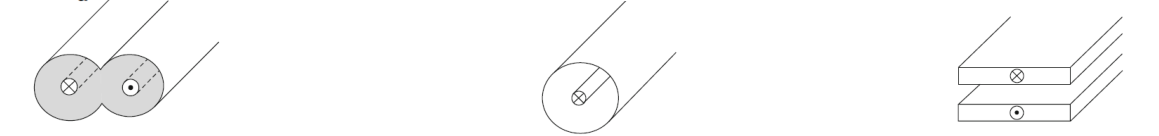
\includegraphics[width=\columnwidth]{Figures/Leitungsparameter.png}

\subsubsection{Doppelleitung:}
\begin{align*}
    a & = \text{Leiter Radius}                   & d & = \text{Abstand zw. den Leitern}                \\
    R & = \frac{1}{\pi a\delta\sigma_c}          & L & = \frac{\mu}{\pi} \cosh^{-1}\frac{d}{2a}      & \\
    G & = \frac{\pi\sigma}{\cosh^{-1}(^d/_{2a})} & C & = \frac{\pi\varepsilon}{\cosh^{-1}(^d/_{2a})}
\end{align*}

\subsubsection{Koaxial Leitung}
\begin{align*}
    a & = \text{innen Radius}                                              & b & = \text{äußerer Radius}               \\
    R & = \frac{1}{2\pi\delta\sigma_c}\left[\frac{1}{a}+\frac{1}{b}\right] & L & = \frac{\mu}{2\pi} \ln\frac{b}{a}     \\
    G & = \frac{2\pi\sigma}{\ln (^b/_a)}                                   & C & = \frac{2\pi\varepsilon}{\ln (^b/_a)}
\end{align*}

\subsubsection{Parallele Platten}
\begin{align*}
    w & = \text{Platten Breite}   & d & = \text{Abstand zw. Platten} \\
    R & = \frac{2}{w\delta\sigma} & L & = \frac{\mu d}{w}            \\
    G & = \frac{\sigma w}{d}      & C & = \frac{w\varepsilon}{d}
\end{align*}

Für beliebige Leitergeometrie gelten folgende Zusammenhänge:
\[
    LC = \mu\varepsilon \quad \text{und} \quad \frac{G}{C} = \frac{\sigma}{\varepsilon}
\]

\subsection{Übertragungsleitung mit Last}

% 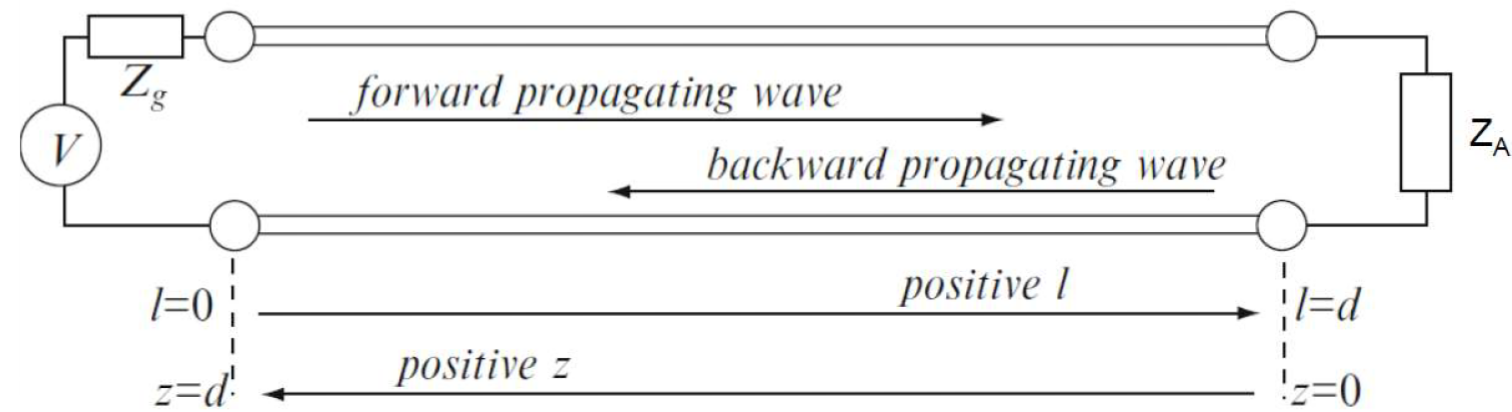
\includegraphics[width=\columnwidth]{Figures/UebertragungleitungmitLast.png}

\vspace{2cm}

\def\Hoehe{2};
\def\Breite{8}
\resizebox{0.4\textwidth}{!}{
    %\centering
    \begin{tikzpicture}
        \begin{circuitikz}%[american voltages]
            \draw(0,0)
            to[V,v=$u_G(t)$](0,2)                           %Spannungsquelle
            to[R=$Z_g$](2,2)                               %Quelleninnenwiderstand
            to[short](8,2)
            to[R= $Z_A$](8,0)                               %Lastwiderstand
            to[short](0,0);             
            \draw[-] (2,2) circle (0.1);                    %TOR 1 oben
            \draw[-] (6,2) circle (0.1);                    %TOR 2 oben
            \draw[-] (2,0) circle (0.1);                    %TOR 1 unten
            \draw[-] (6,0) circle (0.1);                    %TOR 2 unten
            \draw[dotted](2,0)--(2,-0.5) node[left]{$l=0$};
            \draw[dotted](2,-0.5)--(2,-1) node[left]{$z=d$};
            \draw[dotted](2,-1)--(2,-1.5);
            \draw[->](2,-0.5) -- (6,-0.5);
            \node at (5,-0,5)[above]{positiv l};

            \draw[dotted](6,0)--(6,-0.5) node[right]{$l=d$};          
            \draw[dotted](6,-0.5)--(6,-1) node[right]{$z=0$};
            \draw[dotted](6,-1)--(6,-1.5);
            \draw[->](6,-1.5) -- (2,-1.5);
            \node at (5,-1,5)[above]{positiv z};

            \draw[->](2,1.25) -- (5,1.25);
            \node at (4,1.25)[above]{forward propagating wave};
            \draw[->](6,0.5) -- (3,0.5);
            \node at (5,0.5)[above]{backward propagating wave};
        \end{circuitikz}
    \end{tikzpicture}
}

\begin{align*}
    U(z) & = U^+ e^{\gamma z} + U^- e^{-\gamma z} = U^+ e^{\gamma d} + U^ - e^{-\gamma d}                      \\
    I(z) & = I^+ e^{\gamma z} + I^- e^{-\gamma z} = \frac{U^+}{Z_L}e^{\gamma d} - \frac{U^-}{Z_L}e^{-\gamma d}
\end{align*}

\begin{align*}
    \underline{z}_n & = \frac{\underline{Z}_A}{Z_L}                     & \underline{r} & = \frac{\underline{z}_n-1}{\underline{z}_n+1}= \frac{1-\underline{y}_n}{1+\underline{y}_n} \\
    \underline{r}_A & = \frac{\underline{Z}_A-Z_L}{\underline{Z}_A+Z_L} & m             & = \frac{1-|\underline{r}|}{1+|\underline{r}|}
\end{align*}

\subsubsection{Reflexionsfaktor entlang einer Leitung}
\begin{align*}
    r_E    & = r_A  ^{-2\gamma l} = r_A  e^{-2\alpha l} e^{-j2\beta l}                                                     \\
    \alpha & = -\frac{\ln(r_A)}{2l} [\si{Np/m}]                        & \beta & = \dfrac{\phi_2 -\phi_1}{2l} [\si{rad/m}]
\end{align*}

\subsubsection{Stehwellenverhältnis}
\begin{align*}
    \mathrm{SWR} = \frac{U_\text{max}}{U_\text{min}} =
    \frac{I_\text{max}}{I_\text{min}} = \frac{1+|r(z)|}{1-|r(z)|} =
    \frac{|U_H|+|U_R|}{|U_H|-|U_R|}
\end{align*}

\subsection{Mehrfachreflexionen bei fehlender Anpassung}

\begin{center}
    \begin{tikzpicture}
        %Linien
        \draw[-Latex] (1,1) -- (1,0) node [below] {$t$};
        \draw[-,line width=1pt] (1,1) -- (1,6);
        \draw[-,line width=1pt] (5,0) -- (5,6);

        %Pfeile mit Bezeichnungen
        \draw[-Latex] (3.5,6.5) -- (5,6.5)node[right]{$z$};

        \draw[-Latex] (1,6) -- (5,5) node[right]{$t_D$} node[midway, above]{$U_{1h}$};
        %\draw[-] (1,6) -- (3,5.5) node[above]{$U_{1h}$};

        \draw[-Latex] (5,5) -- (1,4)node[left]{$2t_D$} node[midway, above]{$U_{1r}$};
        %\draw[-] (5,5) -- (3,4.5) node[above]{$U_{1r}$};

        \draw[-Latex] (1,4) -- (5,3)node[right]{$3t_D$} node[midway, above]{$U_{2h}$};
        %\draw[-] (1,4) -- (3,3.5) node[above]{$U_{2h}$};

        \draw[-Latex] (5,3) -- (1,2)node[left]{$4t_D$} node[midway, above]{$U_{2r}$};
        %\draw[-] (5,3) -- (3,2.5) node[above]{$U_{2r}$};

        \draw[-Latex] (1,2) -- (5,1)node[right]{$5t_D$} node[midway, above]{$U_{3h}$};
        %\draw[-] (1,2) -- (3,1.5) node[above]{$U_{3h}$};


        \draw[dotted ] (5,1) -- (3,0.5);

        %Klammern mit Bezeichnungen
        \draw [black,
            decorate,
            decoration = {brace,
                    raise=5pt,
                    amplitude=5pt}] (1,4.2) --  (1,5.8);
        \node at(0.5,5)[left]{$U_{1h}$};

        \draw [black,
            decorate,
            decoration = {brace,
                    raise=5pt,
                    amplitude=5pt}] (5,4.8) --  (5,3.2);
        \node at (5.5,4)[right]{$U_{1h}(1+r_A)$};

        \draw [black,
            decorate,
            decoration = {brace,
                    raise=5pt,
                    amplitude=5pt}] (1,2.2) --  (1,3.8);
        \node at (0.5,3)[left]{$U_{1h}$};
        \node at (0.5,2.5)[left]{$+(1+r_I)U_{1r}$};

        \draw [black,
            decorate,
            decoration = {brace,
                    raise=5pt,
                    amplitude=5pt}] (5,2.8) --  (5,1.2);
        \node at (5.5,2)[right]{$U_{1h}(1+r_A)$};
        \node at (5.5,1.5)[right]{$+U_{2h}(1+r_A)$};


        \draw [black,
            decorate,
            decoration = {brace,
                    raise=5pt,
                    amplitude=5pt}] (1,0.2) --  (1,1.8);
        \node at (0.5,1.5)[left]{$U_{1h}$};
        \node at (0.5,1)[left]{$+(1+r_I)U_{1r}$};
        \node at (0.5,0.5)[left]{$+(1+r_I)U_{2r}$};
    \end{tikzpicture}
\end{center}

\begin{align*}
    U_{1h} & = \frac{U_G\cdot Z_L}{R_I + Z_L}            \\
    U_{1r} & = r_A\cdot U_{1h}                           \\
    U_{2h} & = r_I\cdot U_{1r} = r_I\cdot r_A U_{1h}     \\
    U_{2r} & = r_A\cdot U_{2h} = r_I\cdot r_A^2 U_{1h}   \\
    U_{3h} & = r_I\cdot U_{2r} = r_I^2\cdot r_A^2 U_{1h}
\end{align*}
\resizebox{0.4\textwidth}{!}{
    %\centering
    \begin{tikzpicture}
        \begin{circuitikz}%[american voltages]
            \draw(0,0)
            to[V,v=$u_G(t)$](0,2)   %Spannungsquelle
            to[R=$R_I \neq Z_L$](2,2) %Quelleninnenwiderstand
            to[short](8,2)
            to[R= $R_A\neq Z_L$](8,0)
            to[short](0,0)
            (4,2) to [open, v=$u(z\mathpunct{,}t)$] (4,0) %Spannungspfeil u(z,t)
            (2,2) to [open, v=$u_E(t)$] (2,0) %Spannungspfeil u_E(t)
            (6,2) to [open, v=$u_A(t)$] (6,0); %Spannungspfeil u_A(t)
            \draw[-] (2,2) circle (0.1);
            \draw[-] (6,2) circle (0.1);
            \draw[-] (2,0) circle (0.1);
            \draw[-] (6,0) circle (0.1);
        \end{circuitikz}
    \end{tikzpicture}
}
